\documentclass[1p]{elsarticle_modified}
%\bibliographystyle{elsarticle-num}

%\usepackage[colorlinks]{hyperref}
%\usepackage{abbrmath_seonhwa} %\Abb, \Ascr, \Acal ,\Abf, \Afrak
\usepackage{amsfonts}
\usepackage{amssymb}
\usepackage{amsmath}
\usepackage{amsthm}
\usepackage{scalefnt}
\usepackage{amsbsy}
\usepackage{kotex}
\usepackage{caption}
\usepackage{subfig}
\usepackage{color}
\usepackage{graphicx}
\usepackage{xcolor} %% white, black, red, green, blue, cyan, magenta, yellow
\usepackage{float}
\usepackage{setspace}
\usepackage{hyperref}

\usepackage{tikz}
\usetikzlibrary{arrows}

\usepackage{multirow}
\usepackage{array} % fixed length table
\usepackage{hhline}

%%%%%%%%%%%%%%%%%%%%%
\makeatletter
\renewcommand*\env@matrix[1][\arraystretch]{%
	\edef\arraystretch{#1}%
	\hskip -\arraycolsep
	\let\@ifnextchar\new@ifnextchar
	\array{*\c@MaxMatrixCols c}}
\makeatother %https://tex.stackexchange.com/questions/14071/how-can-i-increase-the-line-spacing-in-a-matrix
%%%%%%%%%%%%%%%

\usepackage[normalem]{ulem}

\newcommand{\msout}[1]{\ifmmode\text{\sout{\ensuremath{#1}}}\else\sout{#1}\fi}
%SOURCE: \msout is \stkout macro in https://tex.stackexchange.com/questions/20609/strikeout-in-math-mode

\newcommand{\cancel}[1]{
	\ifmmode
	{\color{red}\msout{#1}}
	\else
	{\color{red}\sout{#1}}
	\fi
}

\newcommand{\add}[1]{
	{\color{blue}\uwave{#1}}
}

\newcommand{\replace}[2]{
	\ifmmode
	{\color{red}\msout{#1}}{\color{blue}\uwave{#2}}
	\else
	{\color{red}\sout{#1}}{\color{blue}\uwave{#2}}
	\fi
}

\newcommand{\Sol}{\mathcal{S}} %segment
\newcommand{\D}{D} %diagram
\newcommand{\A}{\mathcal{A}} %arc


%%%%%%%%%%%%%%%%%%%%%%%%%%%%%5 test

\def\sl{\operatorname{\textup{SL}}(2,\Cbb)}
\def\psl{\operatorname{\textup{PSL}}(2,\Cbb)}
\def\quan{\mkern 1mu \triangleright \mkern 1mu}

\theoremstyle{definition}
\newtheorem{thm}{Theorem}[section]
\newtheorem{prop}[thm]{Proposition}
\newtheorem{lem}[thm]{Lemma}
\newtheorem{ques}[thm]{Question}
\newtheorem{cor}[thm]{Corollary}
\newtheorem{defn}[thm]{Definition}
\newtheorem{exam}[thm]{Example}
\newtheorem{rmk}[thm]{Remark}
\newtheorem{alg}[thm]{Algorithm}

\newcommand{\I}{\sqrt{-1}}
\begin{document}

%\begin{frontmatter}
%
%\title{Boundary parabolic representations of knots up to 8 crossings}
%
%%% Group authors per affiliation:
%\author{Yunhi Cho} 
%\address{Department of Mathematics, University of Seoul, Seoul, Korea}
%\ead{yhcho@uos.ac.kr}
%
%
%\author{Seonhwa Kim} %\fnref{s_kim}}
%\address{Center for Geometry and Physics, Institute for Basic Science, Pohang, 37673, Korea}
%\ead{ryeona17@ibs.re.kr}
%
%\author{Hyuk Kim}
%\address{Department of Mathematical Sciences, Seoul National University, Seoul 08826, Korea}
%\ead{hyukkim@snu.ac.kr}
%
%\author{Seokbeom Yoon}
%\address{Department of Mathematical Sciences, Seoul National University, Seoul, 08826,  Korea}
%\ead{sbyoon15@snu.ac.kr}
%
%\begin{abstract}
%We find all boundary parabolic representation of knots up to 8 crossings.
%
%\end{abstract}
%\begin{keyword}
%    \MSC[2010] 57M25 
%\end{keyword}
%
%\end{frontmatter}

%\linenumbers
%\tableofcontents
%
\newcommand\colored[1]{\textcolor{white}{\rule[-0.35ex]{0.8em}{1.4ex}}\kern-0.8em\color{red} #1}%
%\newcommand\colored[1]{\textcolor{white}{ #1}\kern-2.17ex	\textcolor{white}{ #1}\kern-1.81ex	\textcolor{white}{ #1}\kern-2.15ex\color{red}#1	}

{\Large $\underline{12a_{1000}~(K12a_{1000})}$}

\setlength{\tabcolsep}{10pt}
\renewcommand{\arraystretch}{1.6}
\vspace{1cm}\begin{tabular}{m{100pt}>{\centering\arraybackslash}m{274pt}}
\multirow{5}{120pt}{
	\centering
	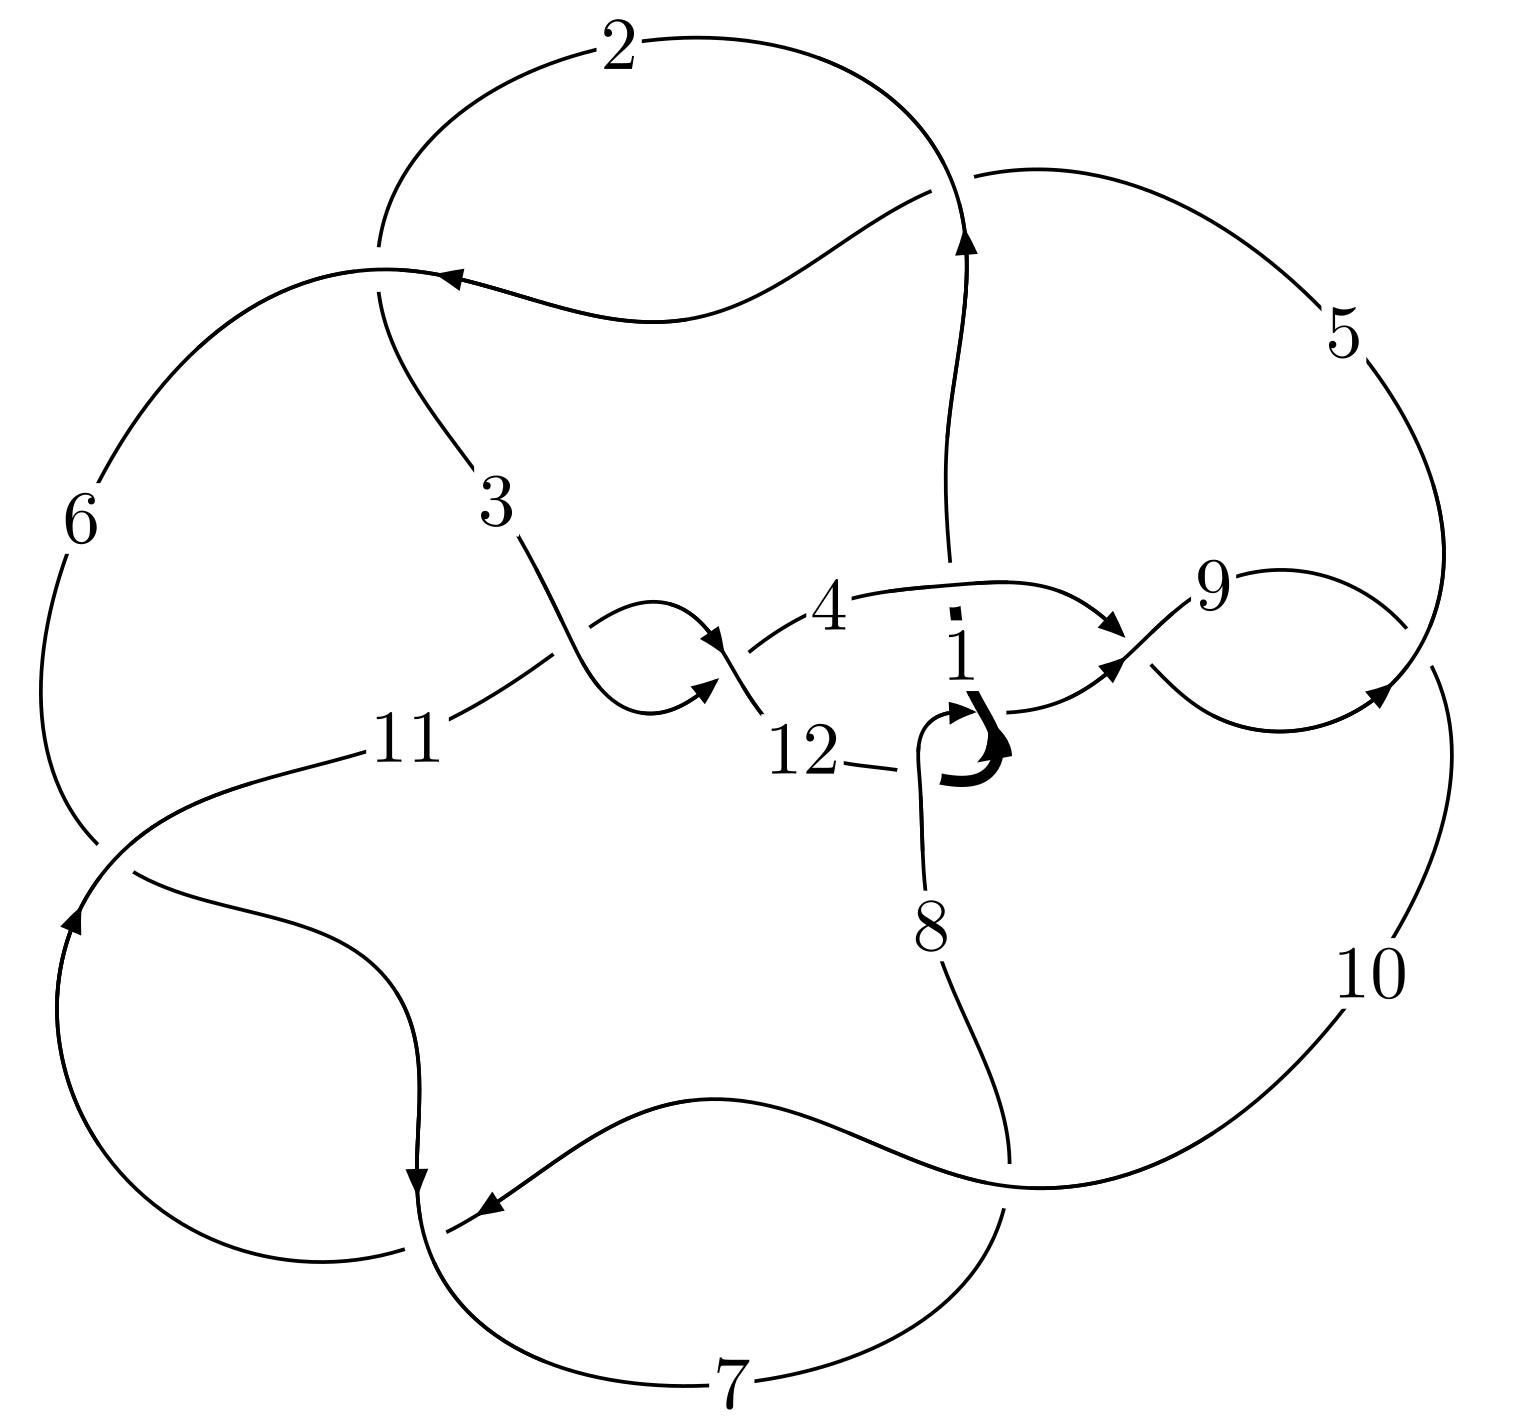
\includegraphics[width=112pt]{../../../GIT/diagram.site/Diagrams/png/1801_12a_1000.png}\\
\ \ \ A knot diagram\footnotemark}&
\allowdisplaybreaks
\textbf{Linearized knot diagam} \\
\cline{2-2}
 &
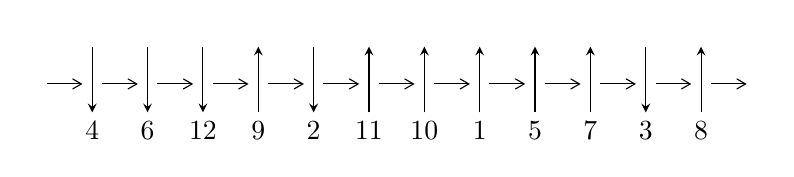
\begin{tikzpicture}[x=20pt, y=17pt]
	% nodes
	\node (C0) at (0, 0) {};
	\node (C1) at (1, 0) {};
	\node (C1U) at (1, +1) {};
	\node (C1D) at (1, -1) {4};

	\node (C2) at (2, 0) {};
	\node (C2U) at (2, +1) {};
	\node (C2D) at (2, -1) {6};

	\node (C3) at (3, 0) {};
	\node (C3U) at (3, +1) {};
	\node (C3D) at (3, -1) {12};

	\node (C4) at (4, 0) {};
	\node (C4U) at (4, +1) {};
	\node (C4D) at (4, -1) {9};

	\node (C5) at (5, 0) {};
	\node (C5U) at (5, +1) {};
	\node (C5D) at (5, -1) {2};

	\node (C6) at (6, 0) {};
	\node (C6U) at (6, +1) {};
	\node (C6D) at (6, -1) {11};

	\node (C7) at (7, 0) {};
	\node (C7U) at (7, +1) {};
	\node (C7D) at (7, -1) {10};

	\node (C8) at (8, 0) {};
	\node (C8U) at (8, +1) {};
	\node (C8D) at (8, -1) {1};

	\node (C9) at (9, 0) {};
	\node (C9U) at (9, +1) {};
	\node (C9D) at (9, -1) {5};

	\node (C10) at (10, 0) {};
	\node (C10U) at (10, +1) {};
	\node (C10D) at (10, -1) {7};

	\node (C11) at (11, 0) {};
	\node (C11U) at (11, +1) {};
	\node (C11D) at (11, -1) {3};

	\node (C12) at (12, 0) {};
	\node (C12U) at (12, +1) {};
	\node (C12D) at (12, -1) {8};
	\node (C13) at (13, 0) {};

	% arrows
	\draw[->,>={angle 60}]
	(C0) edge (C1) (C1) edge (C2) (C2) edge (C3) (C3) edge (C4) (C4) edge (C5) (C5) edge (C6) (C6) edge (C7) (C7) edge (C8) (C8) edge (C9) (C9) edge (C10) (C10) edge (C11) (C11) edge (C12) (C12) edge (C13) ;	\draw[->,>=stealth]
	(C1U) edge (C1D) (C2U) edge (C2D) (C3U) edge (C3D) (C4D) edge (C4U) (C5U) edge (C5D) (C6D) edge (C6U) (C7D) edge (C7U) (C8D) edge (C8U) (C9D) edge (C9U) (C10D) edge (C10U) (C11U) edge (C11D) (C12D) edge (C12U) ;
	\end{tikzpicture} \\
\hhline{~~} \\& 
\textbf{Solving Sequence} \\ \cline{2-2} 
 &
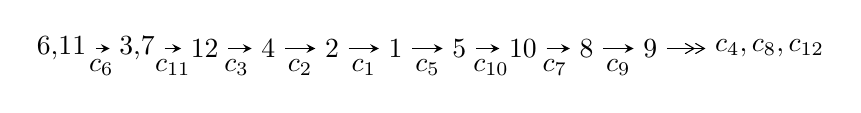
\begin{tikzpicture}[x=23pt, y=7pt]
	% node
	\node (A0) at (-1/8, 0) {6,11};
	\node (A1) at (17/16, 0) {3,7};
	\node (A2) at (17/8, 0) {12};
	\node (A3) at (25/8, 0) {4};
	\node (A4) at (33/8, 0) {2};
	\node (A5) at (41/8, 0) {1};
	\node (A6) at (49/8, 0) {5};
	\node (A7) at (57/8, 0) {10};
	\node (A8) at (65/8, 0) {8};
	\node (A9) at (73/8, 0) {9};
	\node (C1) at (1/2, -1) {$c_{6}$};
	\node (C2) at (13/8, -1) {$c_{11}$};
	\node (C3) at (21/8, -1) {$c_{3}$};
	\node (C4) at (29/8, -1) {$c_{2}$};
	\node (C5) at (37/8, -1) {$c_{1}$};
	\node (C6) at (45/8, -1) {$c_{5}$};
	\node (C7) at (53/8, -1) {$c_{10}$};
	\node (C8) at (61/8, -1) {$c_{7}$};
	\node (C9) at (69/8, -1) {$c_{9}$};
	\node (A10) at (11, 0) {$c_{4},c_{8},c_{12}$};

	% edge
	\draw[->,>=stealth]	
	(A0) edge (A1) (A1) edge (A2) (A2) edge (A3) (A3) edge (A4) (A4) edge (A5) (A5) edge (A6) (A6) edge (A7) (A7) edge (A8) (A8) edge (A9) ;
	\draw[->>,>={angle 60}]	
	(A9) edge (A10);
\end{tikzpicture} \\ 

\end{tabular} \\

\footnotetext{
The image of knot diagram is generated by the software ``\textbf{Draw programme}" developed by Andrew Bartholomew(\url{http://www.layer8.co.uk/maths/draw/index.htm\#Running-draw}), where we modified some parts for our purpose(\url{https://github.com/CATsTAILs/LinksPainter}).
}\phantom \\ \newline 
\centering \textbf{Ideals for irreducible components\footnotemark of $X_{\text{par}}$} 
 
\begin{align*}
I^u_{1}&=\langle 
-507973994943 u^{25}-5311743375735 u^{24}+\cdots+943195983256 b+10737106657608,\\
\phantom{I^u_{1}}&\phantom{= \langle  }1342138332201 u^{25}+13747573664325 u^{24}+\cdots+1886391966512 a-21946395856256,\\
\phantom{I^u_{1}}&\phantom{= \langle  }u^{26}+11 u^{25}+\cdots-96 u-16\rangle \\
I^u_{2}&=\langle 
5 u^{31}-16 u^{30}+\cdots+8 b+64,\;-64 u^{31} a+832 u^{31}+\cdots-928 a+12721,\;u^{32}-4 u^{31}+\cdots+12 u+1\rangle \\
I^u_{3}&=\langle 
-2 u^{12}- u^{10}+25 u^9+60 u^8+123 u^7+200 u^6+228 u^5+255 u^4+210 u^3+144 u^2+17 b+86 u+33,\\
\phantom{I^u_{3}}&\phantom{= \langle  }-33 u^{12}-68 u^{11}+\cdots+17 a-178,\\
\phantom{I^u_{3}}&\phantom{= \langle  }u^{13}+2 u^{12}+9 u^{11}+14 u^{10}+30 u^9+40 u^8+49 u^7+60 u^6+44 u^5+48 u^4+24 u^3+17 u^2+8 u+1\rangle \\
\\
I^v_{1}&=\langle 
a,\;b+1,\;v+1\rangle \\
\end{align*}
\raggedright * 4 irreducible components of $\dim_{\mathbb{C}}=0$, with total 104 representations.\\
\footnotetext{All coefficients of polynomials are rational numbers. But the coefficients are sometimes approximated in decimal forms when there is not enough margin.}
\newpage
\renewcommand{\arraystretch}{1}
\centering \section*{I. $I^u_{1}= \langle -5.08\times10^{11} u^{25}-5.31\times10^{12} u^{24}+\cdots+9.43\times10^{11} b+1.07\times10^{13},\;1.34\times10^{12} u^{25}+1.37\times10^{13} u^{24}+\cdots+1.89\times10^{12} a-2.19\times10^{13},\;u^{26}+11 u^{25}+\cdots-96 u-16 \rangle$}
\flushleft \textbf{(i) Arc colorings}\\
\begin{tabular}{m{7pt} m{180pt} m{7pt} m{180pt} }
\flushright $a_{6}=$&$\begin{pmatrix}1\\0\end{pmatrix}$ \\
\flushright $a_{11}=$&$\begin{pmatrix}0\\u\end{pmatrix}$ \\
\flushright $a_{3}=$&$\begin{pmatrix}-0.711484 u^{25}-7.28776 u^{24}+\cdots+62.9142 u+11.6341\\0.538567 u^{25}+5.63164 u^{24}+\cdots-56.6684 u-11.3837\end{pmatrix}$ \\
\flushright $a_{7}=$&$\begin{pmatrix}1\\- u^2\end{pmatrix}$ \\
\flushright $a_{12}=$&$\begin{pmatrix}0.771582 u^{25}+7.93248 u^{24}+\cdots-61.5071 u-11.9585\\-0.554928 u^{25}-5.84051 u^{24}+\cdots+63.1134 u+12.3453\end{pmatrix}$ \\
\flushright $a_{4}=$&$\begin{pmatrix}-0.170627 u^{25}-1.82922 u^{24}+\cdots+29.2931 u+6.47328\\-0.244914 u^{25}-2.63645 u^{24}+\cdots+30.4117 u+5.88703\end{pmatrix}$ \\
\flushright $a_{2}=$&$\begin{pmatrix}-0.172918 u^{25}-1.65612 u^{24}+\cdots+6.24576 u+0.250310\\0.538567 u^{25}+5.63164 u^{24}+\cdots-56.6684 u-11.3837\end{pmatrix}$ \\
\flushright $a_{1}=$&$\begin{pmatrix}0.503649 u^{25}+5.23569 u^{24}+\cdots-49.7132 u-11.2334\\-0.285246 u^{25}-2.91517 u^{24}+\cdots+26.0137 u+5.17604\end{pmatrix}$ \\
\flushright $a_{5}=$&$\begin{pmatrix}0.216655 u^{25}+2.09197 u^{24}+\cdots+0.606288 u+1.38678\\-0.554928 u^{25}-5.84051 u^{24}+\cdots+62.1134 u+12.3453\end{pmatrix}$ \\
\flushright $a_{10}=$&$\begin{pmatrix}- u\\u^3+u\end{pmatrix}$ \\
\flushright $a_{8}=$&$\begin{pmatrix}u^2+1\\- u^4-2 u^2\end{pmatrix}$ \\
\flushright $a_{9}=$&$\begin{pmatrix}0.0588908 u^{25}+0.409826 u^{24}+\cdots+8.22754 u+2.49800\\-0.437795 u^{25}-4.41833 u^{24}+\cdots+32.6510 u+6.31789\end{pmatrix}$\\&\end{tabular}
\flushleft \textbf{(ii) Obstruction class $= -1$}\\~\\
\flushleft \textbf{(iii) Cusp Shapes $= -\frac{378381583910}{117899497907} u^{25}-\frac{3984664362651}{117899497907} u^{24}+\cdots+\frac{46248892072756}{117899497907} u+\frac{9858826741770}{117899497907}$}\\~\\
\newpage\renewcommand{\arraystretch}{1}
\flushleft \textbf{(iv) u-Polynomials at the component}\newline \\
\begin{tabular}{m{50pt}|m{274pt}}
Crossings & \hspace{64pt}u-Polynomials at each crossing \\
\hline $$\begin{aligned}c_{1}\end{aligned}$$&$\begin{aligned}
&u^{26}-23 u^{25}+\cdots+512 u-256
\end{aligned}$\\
\hline $$\begin{aligned}c_{2},c_{3},c_{5}\\c_{11}\end{aligned}$$&$\begin{aligned}
&u^{26}-14 u^{24}+\cdots-6 u+1
\end{aligned}$\\
\hline $$\begin{aligned}c_{4},c_{8},c_{9}\\c_{12}\end{aligned}$$&$\begin{aligned}
&u^{26}-9 u^{24}+\cdots+3 u+1
\end{aligned}$\\
\hline $$\begin{aligned}c_{6},c_{7},c_{10}\end{aligned}$$&$\begin{aligned}
&u^{26}+11 u^{25}+\cdots-96 u-16
\end{aligned}$\\
\hline
\end{tabular}\\~\\
\newpage\renewcommand{\arraystretch}{1}
\flushleft \textbf{(v) Riley Polynomials at the component}\newline \\
\begin{tabular}{m{50pt}|m{274pt}}
Crossings & \hspace{64pt}Riley Polynomials at each crossing \\
\hline $$\begin{aligned}c_{1}\end{aligned}$$&$\begin{aligned}
&y^{26}-5 y^{25}+\cdots-8060928 y+65536
\end{aligned}$\\
\hline $$\begin{aligned}c_{2},c_{3},c_{5}\\c_{11}\end{aligned}$$&$\begin{aligned}
&y^{26}-28 y^{25}+\cdots-18 y+1
\end{aligned}$\\
\hline $$\begin{aligned}c_{4},c_{8},c_{9}\\c_{12}\end{aligned}$$&$\begin{aligned}
&y^{26}-18 y^{25}+\cdots-13 y+1
\end{aligned}$\\
\hline $$\begin{aligned}c_{6},c_{7},c_{10}\end{aligned}$$&$\begin{aligned}
&y^{26}+23 y^{25}+\cdots+2176 y+256
\end{aligned}$\\
\hline
\end{tabular}\\~\\
\newpage\flushleft \textbf{(vi) Complex Volumes and Cusp Shapes}
$$\begin{array}{c|c|c}  
\text{Solutions to }I^u_{1}& \I (\text{vol} + \sqrt{-1}CS) & \text{Cusp shape}\\
 \hline 
\begin{aligned}
u &= -0.346632 + 0.992789 I \\
a &= \phantom{-}0.455057 - 0.670912 I \\
b &= \phantom{-}0.508337 + 0.684335 I\end{aligned}
 & \phantom{-}4.03470 - 0.73141 I & \phantom{-}5.45646 + 3.23030 I \\ \hline\begin{aligned}
u &= -0.346632 - 0.992789 I \\
a &= \phantom{-}0.455057 + 0.670912 I \\
b &= \phantom{-}0.508337 - 0.684335 I\end{aligned}
 & \phantom{-}4.03470 + 0.73141 I & \phantom{-}5.45646 - 3.23030 I \\ \hline\begin{aligned}
u &= -0.656581 + 0.547695 I \\
a &= -1.13998 - 1.20654 I \\
b &= \phantom{-}1.40930 + 0.16783 I\end{aligned}
 & -7.54501 - 2.22964 I & -6.88659 + 1.47861 I \\ \hline\begin{aligned}
u &= -0.656581 - 0.547695 I \\
a &= -1.13998 + 1.20654 I \\
b &= \phantom{-}1.40930 - 0.16783 I\end{aligned}
 & -7.54501 + 2.22964 I & -6.88659 - 1.47861 I \\ \hline\begin{aligned}
u &= -1.012690 + 0.638363 I \\
a &= \phantom{-}0.831253 + 0.884931 I \\
b &= -1.40671 - 0.36552 I\end{aligned}
 & -0.71270 - 12.30050 I & \phantom{-}0.84803 + 8.11656 I \\ \hline\begin{aligned}
u &= -1.012690 - 0.638363 I \\
a &= \phantom{-}0.831253 - 0.884931 I \\
b &= -1.40671 + 0.36552 I\end{aligned}
 & -0.71270 + 12.30050 I & \phantom{-}0.84803 - 8.11656 I \\ \hline\begin{aligned}
u &= -0.717925 + 0.120399 I \\
a &= -0.520959 + 0.998156 I \\
b &= \phantom{-}0.253833 - 0.779324 I\end{aligned}
 & \phantom{-}6.67762 - 3.08794 I & \phantom{-}9.21380 + 1.80971 I \\ \hline\begin{aligned}
u &= -0.717925 - 0.120399 I \\
a &= -0.520959 - 0.998156 I \\
b &= \phantom{-}0.253833 + 0.779324 I\end{aligned}
 & \phantom{-}6.67762 + 3.08794 I & \phantom{-}9.21380 - 1.80971 I \\ \hline\begin{aligned}
u &= -1.28198\phantom{ +0.000000I} \\
a &= -1.13116\phantom{ +0.000000I} \\
b &= \phantom{-}1.45012\phantom{ +0.000000I}\end{aligned}
 & -4.99672\phantom{ +0.000000I} & \phantom{-}2.97320\phantom{ +0.000000I} \\ \hline\begin{aligned}
u &= \phantom{-}0.126944 + 1.295060 I \\
a &= \phantom{-}0.265595 - 0.087832 I \\
b &= \phantom{-}0.147463 + 0.332812 I\end{aligned}
 & -3.35359 + 2.09018 I & \phantom{-}5.38222 - 3.50453 I\\
 \hline 
 \end{array}$$\newpage$$\begin{array}{c|c|c}  
\text{Solutions to }I^u_{1}& \I (\text{vol} + \sqrt{-1}CS) & \text{Cusp shape}\\
 \hline 
\begin{aligned}
u &= \phantom{-}0.126944 - 1.295060 I \\
a &= \phantom{-}0.265595 + 0.087832 I \\
b &= \phantom{-}0.147463 - 0.332812 I\end{aligned}
 & -3.35359 - 2.09018 I & \phantom{-}5.38222 + 3.50453 I \\ \hline\begin{aligned}
u &= -0.309354 + 1.290100 I \\
a &= -0.511022 + 0.072506 I \\
b &= \phantom{-}0.064546 - 0.681699 I\end{aligned}
 & \phantom{-}2.31636 - 6.78533 I & \phantom{-}4.90741 + 2.92210 I \\ \hline\begin{aligned}
u &= -0.309354 - 1.290100 I \\
a &= -0.511022 - 0.072506 I \\
b &= \phantom{-}0.064546 + 0.681699 I\end{aligned}
 & \phantom{-}2.31636 + 6.78533 I & \phantom{-}4.90741 - 2.92210 I \\ \hline\begin{aligned}
u &= -1.082260 + 0.813357 I \\
a &= \phantom{-}0.813423 + 0.519935 I \\
b &= -1.303230 + 0.098901 I\end{aligned}
 & -1.01017 + 5.35308 I & \phantom{-0.000000 } 0. - 4.95781 I \\ \hline\begin{aligned}
u &= -1.082260 - 0.813357 I \\
a &= \phantom{-}0.813423 - 0.519935 I \\
b &= -1.303230 - 0.098901 I\end{aligned}
 & -1.01017 - 5.35308 I & \phantom{-0.000000 -}0. + 4.95781 I \\ \hline\begin{aligned}
u &= \phantom{-}0.492337\phantom{ +0.000000I} \\
a &= \phantom{-}0.403546\phantom{ +0.000000I} \\
b &= \phantom{-}0.198681\phantom{ +0.000000I}\end{aligned}
 & \phantom{-}0.832719\phantom{ +0.000000I} & \phantom{-}12.0990\phantom{ +0.000000I} \\ \hline\begin{aligned}
u &= -0.20866 + 1.55520 I \\
a &= \phantom{-}0.155152 - 1.028070 I \\
b &= \phantom{-}1.56648 + 0.45581 I\end{aligned}
 & -14.5475 - 5.3956 I & \phantom{-0.000000 } 0 \\ \hline\begin{aligned}
u &= -0.20866 - 1.55520 I \\
a &= \phantom{-}0.155152 + 1.028070 I \\
b &= \phantom{-}1.56648 - 0.45581 I\end{aligned}
 & -14.5475 + 5.3956 I & \phantom{-0.000000 } 0 \\ \hline\begin{aligned}
u &= \phantom{-}0.109643 + 0.356252 I \\
a &= -0.85111 + 1.69328 I \\
b &= -0.696554 - 0.117553 I\end{aligned}
 & -1.288240 - 0.193189 I & -7.14857 + 0.44493 I \\ \hline\begin{aligned}
u &= \phantom{-}0.109643 - 0.356252 I \\
a &= -0.85111 - 1.69328 I \\
b &= -0.696554 + 0.117553 I\end{aligned}
 & -1.288240 + 0.193189 I & -7.14857 - 0.44493 I\\
 \hline 
 \end{array}$$\newpage$$\begin{array}{c|c|c}  
\text{Solutions to }I^u_{1}& \I (\text{vol} + \sqrt{-1}CS) & \text{Cusp shape}\\
 \hline 
\begin{aligned}
u &= -0.33614 + 1.61309 I \\
a &= -0.128911 + 1.022060 I \\
b &= -1.60534 - 0.55150 I\end{aligned}
 & -8.0518 - 17.2435 I & \phantom{-0.000000 } 0 \\ \hline\begin{aligned}
u &= -0.33614 - 1.61309 I \\
a &= -0.128911 - 1.022060 I \\
b &= -1.60534 + 0.55150 I\end{aligned}
 & -8.0518 + 17.2435 I & \phantom{-0.000000 } 0 \\ \hline\begin{aligned}
u &= -0.51814 + 1.56536 I \\
a &= -0.133329 - 0.923680 I \\
b &= \phantom{-}1.51497 + 0.26989 I\end{aligned}
 & -10.19140 - 6.55039 I & \phantom{-0.000000 } 0 \\ \hline\begin{aligned}
u &= -0.51814 - 1.56536 I \\
a &= -0.133329 + 0.923680 I \\
b &= \phantom{-}1.51497 - 0.26989 I\end{aligned}
 & -10.19140 + 6.55039 I & \phantom{-0.000000 } 0 \\ \hline\begin{aligned}
u &= -0.15338 + 1.72340 I \\
a &= -0.121371 + 0.752073 I \\
b &= -1.277510 - 0.324523 I\end{aligned}
 & -10.30440 + 0.51735 I & \phantom{-0.000000 } 0 \\ \hline\begin{aligned}
u &= -0.15338 - 1.72340 I \\
a &= -0.121371 - 0.752073 I \\
b &= -1.277510 + 0.324523 I\end{aligned}
 & -10.30440 - 0.51735 I & \phantom{-0.000000 } 0\\
 \hline 
 \end{array}$$\newpage\newpage\renewcommand{\arraystretch}{1}
\centering \section*{II. $I^u_{2}= \langle 5 u^{31}-16 u^{30}+\cdots+8 b+64,\;-64 u^{31} a+832 u^{31}+\cdots-928 a+12721,\;u^{32}-4 u^{31}+\cdots+12 u+1 \rangle$}
\flushleft \textbf{(i) Arc colorings}\\
\begin{tabular}{m{7pt} m{180pt} m{7pt} m{180pt} }
\flushright $a_{6}=$&$\begin{pmatrix}1\\0\end{pmatrix}$ \\
\flushright $a_{11}=$&$\begin{pmatrix}0\\u\end{pmatrix}$ \\
\flushright $a_{3}=$&$\begin{pmatrix}a\\-\frac{5}{8} u^{31}+2 u^{30}+\cdots+20 u-8\end{pmatrix}$ \\
\flushright $a_{7}=$&$\begin{pmatrix}1\\- u^2\end{pmatrix}$ \\
\flushright $a_{12}=$&$\begin{pmatrix}\frac{5}{8} u^{31} a-7 u^{31}+\cdots+8 a-104\\- u^{31}+\frac{31}{8} u^{30}+\cdots+21 u-7\end{pmatrix}$ \\
\flushright $a_{4}=$&$\begin{pmatrix}-\frac{25}{8} u^{31} a+\frac{515}{8} u^{31}+\cdots-64 a+1002\\-\frac{1}{8} u^{31} a-\frac{5}{8} u^{31}+\cdots+a-8\end{pmatrix}$ \\
\flushright $a_{2}=$&$\begin{pmatrix}-\frac{5}{8} u^{31}+2 u^{30}+\cdots+a-8\\-\frac{5}{8} u^{31}+2 u^{30}+\cdots+20 u-8\end{pmatrix}$ \\
\flushright $a_{1}=$&$\begin{pmatrix}u^{31} a-8 u^{31}+\cdots+\frac{65}{8} a-112\\\frac{1}{8} u^{31} a- u^{31}+\cdots+\frac{1}{8} a-7\end{pmatrix}$ \\
\flushright $a_{5}=$&$\begin{pmatrix}-\frac{1}{2} u^{31} a+\frac{31}{8} u^{31}+\cdots+\frac{5}{8} a+40\\-\frac{1}{2} u^{31} a-\frac{25}{8} u^{31}+\cdots+\frac{5}{8} a-65\end{pmatrix}$ \\
\flushright $a_{10}=$&$\begin{pmatrix}- u\\u^3+u\end{pmatrix}$ \\
\flushright $a_{8}=$&$\begin{pmatrix}u^2+1\\- u^4-2 u^2\end{pmatrix}$ \\
\flushright $a_{9}=$&$\begin{pmatrix}-\frac{1}{2} u^{31} a-\frac{81}{8} u^{31}+\cdots+\frac{17}{2} a-170\\-0.500000 a u^{31}+5.25000 u^{31}+\cdots-194.625 u+69.3750\end{pmatrix}$\\&\end{tabular}
\flushleft \textbf{(ii) Obstruction class $= -1$}\\~\\
\flushleft \textbf{(iii) Cusp Shapes $= \frac{195}{2} u^{31}-384 u^{30}+\cdots-4750 u+1496$}\\~\\
\newpage\renewcommand{\arraystretch}{1}
\flushleft \textbf{(iv) u-Polynomials at the component}\newline \\
\begin{tabular}{m{50pt}|m{274pt}}
Crossings & \hspace{64pt}u-Polynomials at each crossing \\
\hline $$\begin{aligned}c_{1}\end{aligned}$$&$\begin{aligned}
&(u^{32}+6 u^{31}+\cdots+12 u+1)^{2}
\end{aligned}$\\
\hline $$\begin{aligned}c_{2},c_{3},c_{5}\\c_{11}\end{aligned}$$&$\begin{aligned}
&u^{64}+5 u^{63}+\cdots+37990 u+2243
\end{aligned}$\\
\hline $$\begin{aligned}c_{4},c_{8},c_{9}\\c_{12}\end{aligned}$$&$\begin{aligned}
&u^{64}+15 u^{63}+\cdots+1020 u+389
\end{aligned}$\\
\hline $$\begin{aligned}c_{6},c_{7},c_{10}\end{aligned}$$&$\begin{aligned}
&(u^{32}-4 u^{31}+\cdots+12 u+1)^{2}
\end{aligned}$\\
\hline
\end{tabular}\\~\\
\newpage\renewcommand{\arraystretch}{1}
\flushleft \textbf{(v) Riley Polynomials at the component}\newline \\
\begin{tabular}{m{50pt}|m{274pt}}
Crossings & \hspace{64pt}Riley Polynomials at each crossing \\
\hline $$\begin{aligned}c_{1}\end{aligned}$$&$\begin{aligned}
&(y^{32}+8 y^{31}+\cdots-80 y+1)^{2}
\end{aligned}$\\
\hline $$\begin{aligned}c_{2},c_{3},c_{5}\\c_{11}\end{aligned}$$&$\begin{aligned}
&y^{64}-125 y^{63}+\cdots-105577704 y+5031049
\end{aligned}$\\
\hline $$\begin{aligned}c_{4},c_{8},c_{9}\\c_{12}\end{aligned}$$&$\begin{aligned}
&y^{64}-113 y^{63}+\cdots+2826260 y+151321
\end{aligned}$\\
\hline $$\begin{aligned}c_{6},c_{7},c_{10}\end{aligned}$$&$\begin{aligned}
&(y^{32}+36 y^{31}+\cdots-224 y+1)^{2}
\end{aligned}$\\
\hline
\end{tabular}\\~\\
\newpage\flushleft \textbf{(vi) Complex Volumes and Cusp Shapes}
$$\begin{array}{c|c|c}  
\text{Solutions to }I^u_{2}& \I (\text{vol} + \sqrt{-1}CS) & \text{Cusp shape}\\
 \hline 
\begin{aligned}
u &= -0.431291 + 0.935489 I \\
a &= -0.956425 - 0.649337 I \\
b &= -0.249448 - 0.237320 I\end{aligned}
 & \phantom{-}2.64508 + 4.13131 I & \phantom{-}2.00000 - 1.07938 I \\ \hline\begin{aligned}
u &= -0.431291 + 0.935489 I \\
a &= -0.107831 + 0.316363 I \\
b &= \phantom{-}1.019950 - 0.614672 I\end{aligned}
 & \phantom{-}2.64508 + 4.13131 I & \phantom{-}2.00000 - 1.07938 I \\ \hline\begin{aligned}
u &= -0.431291 - 0.935489 I \\
a &= -0.956425 + 0.649337 I \\
b &= -0.249448 + 0.237320 I\end{aligned}
 & \phantom{-}2.64508 - 4.13131 I & \phantom{-}2.00000 + 1.07938 I \\ \hline\begin{aligned}
u &= -0.431291 - 0.935489 I \\
a &= -0.107831 - 0.316363 I \\
b &= \phantom{-}1.019950 + 0.614672 I\end{aligned}
 & \phantom{-}2.64508 - 4.13131 I & \phantom{-}2.00000 + 1.07938 I \\ \hline\begin{aligned}
u &= \phantom{-}0.772766 + 0.711176 I \\
a &= \phantom{-}0.805503 - 1.026110 I \\
b &= -1.37402 + 0.41443 I\end{aligned}
 & -4.52142 + 6.63284 I & -2.00159 - 6.22856 I \\ \hline\begin{aligned}
u &= \phantom{-}0.772766 + 0.711176 I \\
a &= -0.695473 + 1.176340 I \\
b &= \phantom{-}1.352210 - 0.220085 I\end{aligned}
 & -4.52142 + 6.63284 I & -2.00159 - 6.22856 I \\ \hline\begin{aligned}
u &= \phantom{-}0.772766 - 0.711176 I \\
a &= \phantom{-}0.805503 + 1.026110 I \\
b &= -1.37402 - 0.41443 I\end{aligned}
 & -4.52142 - 6.63284 I & -2.00159 + 6.22856 I \\ \hline\begin{aligned}
u &= \phantom{-}0.772766 - 0.711176 I \\
a &= -0.695473 - 1.176340 I \\
b &= \phantom{-}1.352210 + 0.220085 I\end{aligned}
 & -4.52142 - 6.63284 I & -2.00159 + 6.22856 I \\ \hline\begin{aligned}
u &= \phantom{-}1.042100 + 0.409476 I \\
a &= -1.038010 + 0.351756 I \\
b &= \phantom{-}1.379790 - 0.010337 I\end{aligned}
 & -3.43055 - 0.83324 I & \phantom{-0.000000 } 0 \\ \hline\begin{aligned}
u &= \phantom{-}1.042100 + 0.409476 I \\
a &= \phantom{-}1.143580 - 0.459271 I \\
b &= -1.225740 - 0.058473 I\end{aligned}
 & -3.43055 - 0.83324 I & \phantom{-0.000000 } 0\\
 \hline 
 \end{array}$$\newpage$$\begin{array}{c|c|c}  
\text{Solutions to }I^u_{2}& \I (\text{vol} + \sqrt{-1}CS) & \text{Cusp shape}\\
 \hline 
\begin{aligned}
u &= \phantom{-}1.042100 - 0.409476 I \\
a &= -1.038010 - 0.351756 I \\
b &= \phantom{-}1.379790 + 0.010337 I\end{aligned}
 & -3.43055 + 0.83324 I & \phantom{-0.000000 } 0 \\ \hline\begin{aligned}
u &= \phantom{-}1.042100 - 0.409476 I \\
a &= \phantom{-}1.143580 + 0.459271 I \\
b &= -1.225740 + 0.058473 I\end{aligned}
 & -3.43055 + 0.83324 I & \phantom{-0.000000 } 0 \\ \hline\begin{aligned}
u &= \phantom{-}0.396831 + 0.630762 I \\
a &= \phantom{-}0.541000 + 0.721874 I \\
b &= \phantom{-}0.905643 - 0.460146 I\end{aligned}
 & \phantom{-}0.45224 + 3.64045 I & \phantom{-}2.24261 - 7.23107 I \\ \hline\begin{aligned}
u &= \phantom{-}0.396831 + 0.630762 I \\
a &= \phantom{-}0.124510 - 1.357460 I \\
b &= -0.240645 + 0.627704 I\end{aligned}
 & \phantom{-}0.45224 + 3.64045 I & \phantom{-}2.24261 - 7.23107 I \\ \hline\begin{aligned}
u &= \phantom{-}0.396831 - 0.630762 I \\
a &= \phantom{-}0.541000 - 0.721874 I \\
b &= \phantom{-}0.905643 + 0.460146 I\end{aligned}
 & \phantom{-}0.45224 - 3.64045 I & \phantom{-}2.24261 + 7.23107 I \\ \hline\begin{aligned}
u &= \phantom{-}0.396831 - 0.630762 I \\
a &= \phantom{-}0.124510 + 1.357460 I \\
b &= -0.240645 - 0.627704 I\end{aligned}
 & \phantom{-}0.45224 - 3.64045 I & \phantom{-}2.24261 + 7.23107 I \\ \hline\begin{aligned}
u &= -0.539207 + 0.347535 I \\
a &= \phantom{-}0.63868 - 1.40504 I \\
b &= \phantom{-}1.059540 + 0.479611 I\end{aligned}
 & \phantom{-}4.27736 - 7.62552 I & \phantom{-}5.45701 + 7.52207 I \\ \hline\begin{aligned}
u &= -0.539207 + 0.347535 I \\
a &= -0.98325 - 1.52321 I \\
b &= \phantom{-}0.143917 + 0.979573 I\end{aligned}
 & \phantom{-}4.27736 - 7.62552 I & \phantom{-}5.45701 + 7.52207 I \\ \hline\begin{aligned}
u &= -0.539207 - 0.347535 I \\
a &= \phantom{-}0.63868 + 1.40504 I \\
b &= \phantom{-}1.059540 - 0.479611 I\end{aligned}
 & \phantom{-}4.27736 + 7.62552 I & \phantom{-}5.45701 - 7.52207 I \\ \hline\begin{aligned}
u &= -0.539207 - 0.347535 I \\
a &= -0.98325 + 1.52321 I \\
b &= \phantom{-}0.143917 - 0.979573 I\end{aligned}
 & \phantom{-}4.27736 + 7.62552 I & \phantom{-}5.45701 - 7.52207 I\\
 \hline 
 \end{array}$$\newpage$$\begin{array}{c|c|c}  
\text{Solutions to }I^u_{2}& \I (\text{vol} + \sqrt{-1}CS) & \text{Cusp shape}\\
 \hline 
\begin{aligned}
u &= -0.582148\phantom{ +0.000000I} \\
a &= \phantom{-}0.662437\phantom{ +0.000000I} \\
b &= -1.33289\phantom{ +0.000000I}\end{aligned}
 & \phantom{-}0.971767\phantom{ +0.000000I} & \phantom{-}9.58410\phantom{ +0.000000I} \\ \hline\begin{aligned}
u &= -0.582148\phantom{ +0.000000I} \\
a &= \phantom{-}2.28961\phantom{ +0.000000I} \\
b &= -0.385636\phantom{ +0.000000I}\end{aligned}
 & \phantom{-}0.971767\phantom{ +0.000000I} & \phantom{-}9.58410\phantom{ +0.000000I} \\ \hline\begin{aligned}
u &= \phantom{-}0.490519 + 0.301188 I \\
a &= \phantom{-}1.53553 + 0.29469 I \\
b &= -0.178851 - 0.166315 I\end{aligned}
 & \phantom{-}1.47460 - 0.45386 I & \phantom{-}7.73807 - 0.08751 I \\ \hline\begin{aligned}
u &= \phantom{-}0.490519 + 0.301188 I \\
a &= -0.415975 - 0.083643 I \\
b &= \phantom{-}0.664449 + 0.607034 I\end{aligned}
 & \phantom{-}1.47460 - 0.45386 I & \phantom{-}7.73807 - 0.08751 I \\ \hline\begin{aligned}
u &= \phantom{-}0.490519 - 0.301188 I \\
a &= \phantom{-}1.53553 - 0.29469 I \\
b &= -0.178851 + 0.166315 I\end{aligned}
 & \phantom{-}1.47460 + 0.45386 I & \phantom{-}7.73807 + 0.08751 I \\ \hline\begin{aligned}
u &= \phantom{-}0.490519 - 0.301188 I \\
a &= -0.415975 + 0.083643 I \\
b &= \phantom{-}0.664449 - 0.607034 I\end{aligned}
 & \phantom{-}1.47460 + 0.45386 I & \phantom{-}7.73807 + 0.08751 I \\ \hline\begin{aligned}
u &= -0.18830 + 1.42349 I \\
a &= \phantom{-}0.202038 + 1.104330 I \\
b &= -0.414850 - 0.754593 I\end{aligned}
 & -3.83881 - 2.75921 I & \phantom{-0.000000 } 0 \\ \hline\begin{aligned}
u &= -0.18830 + 1.42349 I \\
a &= -0.483097 + 0.355334 I \\
b &= -1.61005 + 0.07966 I\end{aligned}
 & -3.83881 - 2.75921 I & \phantom{-0.000000 } 0 \\ \hline\begin{aligned}
u &= -0.18830 - 1.42349 I \\
a &= \phantom{-}0.202038 - 1.104330 I \\
b &= -0.414850 + 0.754593 I\end{aligned}
 & -3.83881 + 2.75921 I & \phantom{-0.000000 } 0 \\ \hline\begin{aligned}
u &= -0.18830 - 1.42349 I \\
a &= -0.483097 - 0.355334 I \\
b &= -1.61005 - 0.07966 I\end{aligned}
 & -3.83881 + 2.75921 I & \phantom{-0.000000 } 0\\
 \hline 
 \end{array}$$\newpage$$\begin{array}{c|c|c}  
\text{Solutions to }I^u_{2}& \I (\text{vol} + \sqrt{-1}CS) & \text{Cusp shape}\\
 \hline 
\begin{aligned}
u &= \phantom{-}0.03982 + 1.44524 I \\
a &= \phantom{-}0.057513 + 0.785575 I \\
b &= \phantom{-}2.64086 - 2.38897 I\end{aligned}
 & -5.23105 + 0.39376 I & \phantom{-0.000000 } 0 \\ \hline\begin{aligned}
u &= \phantom{-}0.03982 + 1.44524 I \\
a &= -1.60143 - 1.87142 I \\
b &= -1.133050 + 0.114406 I\end{aligned}
 & -5.23105 + 0.39376 I & \phantom{-0.000000 } 0 \\ \hline\begin{aligned}
u &= \phantom{-}0.03982 - 1.44524 I \\
a &= \phantom{-}0.057513 - 0.785575 I \\
b &= \phantom{-}2.64086 + 2.38897 I\end{aligned}
 & -5.23105 - 0.39376 I & \phantom{-0.000000 } 0 \\ \hline\begin{aligned}
u &= \phantom{-}0.03982 - 1.44524 I \\
a &= -1.60143 + 1.87142 I \\
b &= -1.133050 - 0.114406 I\end{aligned}
 & -5.23105 - 0.39376 I & \phantom{-0.000000 } 0 \\ \hline\begin{aligned}
u &= \phantom{-}0.09697 + 1.46165 I \\
a &= \phantom{-}0.395493 - 0.884437 I \\
b &= -0.410137 + 0.605887 I\end{aligned}
 & -4.24943 + 1.41411 I & \phantom{-0.000000 } 0 \\ \hline\begin{aligned}
u &= \phantom{-}0.09697 + 1.46165 I \\
a &= \phantom{-}0.394172 + 0.306749 I \\
b &= \phantom{-}1.33109 + 0.49231 I\end{aligned}
 & -4.24943 + 1.41411 I & \phantom{-0.000000 } 0 \\ \hline\begin{aligned}
u &= \phantom{-}0.09697 - 1.46165 I \\
a &= \phantom{-}0.395493 + 0.884437 I \\
b &= -0.410137 - 0.605887 I\end{aligned}
 & -4.24943 - 1.41411 I & \phantom{-0.000000 } 0 \\ \hline\begin{aligned}
u &= \phantom{-}0.09697 - 1.46165 I \\
a &= \phantom{-}0.394172 - 0.306749 I \\
b &= \phantom{-}1.33109 - 0.49231 I\end{aligned}
 & -4.24943 - 1.41411 I & \phantom{-0.000000 } 0 \\ \hline\begin{aligned}
u &= \phantom{-}0.076052 + 0.502619 I \\
a &= -0.01589 + 1.53409 I \\
b &= -0.789172 - 0.391993 I\end{aligned}
 & -1.275510 - 0.126168 I & -6.13877 - 0.17917 I \\ \hline\begin{aligned}
u &= \phantom{-}0.076052 + 0.502619 I \\
a &= -0.99470 + 1.41961 I \\
b &= -0.772271 + 0.108685 I\end{aligned}
 & -1.275510 - 0.126168 I & -6.13877 - 0.17917 I\\
 \hline 
 \end{array}$$\newpage$$\begin{array}{c|c|c}  
\text{Solutions to }I^u_{2}& \I (\text{vol} + \sqrt{-1}CS) & \text{Cusp shape}\\
 \hline 
\begin{aligned}
u &= \phantom{-}0.076052 - 0.502619 I \\
a &= -0.01589 - 1.53409 I \\
b &= -0.789172 + 0.391993 I\end{aligned}
 & -1.275510 + 0.126168 I & -6.13877 + 0.17917 I \\ \hline\begin{aligned}
u &= \phantom{-}0.076052 - 0.502619 I \\
a &= -0.99470 - 1.41961 I \\
b &= -0.772271 - 0.108685 I\end{aligned}
 & -1.275510 + 0.126168 I & -6.13877 + 0.17917 I \\ \hline\begin{aligned}
u &= -0.15788 + 1.49111 I \\
a &= \phantom{-}0.990763 - 0.348619 I \\
b &= \phantom{-}1.334190 + 0.255540 I\end{aligned}
 & -1.85151 - 10.06120 I & \phantom{-0.000000 } 0 \\ \hline\begin{aligned}
u &= -0.15788 + 1.49111 I \\
a &= \phantom{-}0.075786 - 0.902790 I \\
b &= \phantom{-}0.36340 + 1.53238 I\end{aligned}
 & -1.85151 - 10.06120 I & \phantom{-0.000000 } 0 \\ \hline\begin{aligned}
u &= -0.15788 - 1.49111 I \\
a &= \phantom{-}0.990763 + 0.348619 I \\
b &= \phantom{-}1.334190 - 0.255540 I\end{aligned}
 & -1.85151 + 10.06120 I & \phantom{-0.000000 } 0 \\ \hline\begin{aligned}
u &= -0.15788 - 1.49111 I \\
a &= \phantom{-}0.075786 + 0.902790 I \\
b &= \phantom{-}0.36340 - 1.53238 I\end{aligned}
 & -1.85151 + 10.06120 I & \phantom{-0.000000 } 0 \\ \hline\begin{aligned}
u &= \phantom{-}0.03260 + 1.52702 I \\
a &= -0.105052 + 0.896857 I \\
b &= -0.468227 - 1.029110 I\end{aligned}
 & -8.11506 + 0.32962 I & \phantom{-0.000000 } 0 \\ \hline\begin{aligned}
u &= \phantom{-}0.03260 + 1.52702 I \\
a &= -0.680170 + 0.292106 I \\
b &= -1.372940 - 0.131175 I\end{aligned}
 & -8.11506 + 0.32962 I & \phantom{-0.000000 } 0 \\ \hline\begin{aligned}
u &= \phantom{-}0.03260 - 1.52702 I \\
a &= -0.105052 - 0.896857 I \\
b &= -0.468227 + 1.029110 I\end{aligned}
 & -8.11506 - 0.32962 I & \phantom{-0.000000 } 0 \\ \hline\begin{aligned}
u &= \phantom{-}0.03260 - 1.52702 I \\
a &= -0.680170 - 0.292106 I \\
b &= -1.372940 + 0.131175 I\end{aligned}
 & -8.11506 - 0.32962 I & \phantom{-0.000000 } 0\\
 \hline 
 \end{array}$$\newpage$$\begin{array}{c|c|c}  
\text{Solutions to }I^u_{2}& \I (\text{vol} + \sqrt{-1}CS) & \text{Cusp shape}\\
 \hline 
\begin{aligned}
u &= \phantom{-}0.07478 + 1.55930 I \\
a &= -0.126779 - 0.865817 I \\
b &= -0.175645 + 0.991240 I\end{aligned}
 & -6.95948 + 5.18070 I & \phantom{-0.000000 } 0 \\ \hline\begin{aligned}
u &= \phantom{-}0.07478 + 1.55930 I \\
a &= \phantom{-}0.628848 + 0.142802 I \\
b &= \phantom{-}1.340590 - 0.262433 I\end{aligned}
 & -6.95948 + 5.18070 I & \phantom{-0.000000 } 0 \\ \hline\begin{aligned}
u &= \phantom{-}0.07478 - 1.55930 I \\
a &= -0.126779 + 0.865817 I \\
b &= -0.175645 - 0.991240 I\end{aligned}
 & -6.95948 - 5.18070 I & \phantom{-0.000000 } 0 \\ \hline\begin{aligned}
u &= \phantom{-}0.07478 - 1.55930 I \\
a &= \phantom{-}0.628848 - 0.142802 I \\
b &= \phantom{-}1.340590 + 0.262433 I\end{aligned}
 & -6.95948 - 5.18070 I & \phantom{-0.000000 } 0 \\ \hline\begin{aligned}
u &= \phantom{-}0.24956 + 1.60155 I \\
a &= -0.136197 - 0.928161 I \\
b &= -1.67985 + 0.63113 I\end{aligned}
 & -12.1519 + 10.4459 I & \phantom{-0.000000 } 0 \\ \hline\begin{aligned}
u &= \phantom{-}0.24956 + 1.60155 I \\
a &= \phantom{-}0.225165 + 1.083980 I \\
b &= \phantom{-}1.45251 - 0.44976 I\end{aligned}
 & -12.1519 + 10.4459 I & \phantom{-0.000000 } 0 \\ \hline\begin{aligned}
u &= \phantom{-}0.24956 - 1.60155 I \\
a &= -0.136197 + 0.928161 I \\
b &= -1.67985 - 0.63113 I\end{aligned}
 & -12.1519 - 10.4459 I & \phantom{-0.000000 } 0 \\ \hline\begin{aligned}
u &= \phantom{-}0.24956 - 1.60155 I \\
a &= \phantom{-}0.225165 - 1.083980 I \\
b &= \phantom{-}1.45251 + 0.44976 I\end{aligned}
 & -12.1519 - 10.4459 I & \phantom{-0.000000 } 0 \\ \hline\begin{aligned}
u &= \phantom{-}0.36857 + 1.67271 I \\
a &= \phantom{-}0.037760 - 0.877985 I \\
b &= -1.219860 + 0.318063 I\end{aligned}
 & -10.34730 + 4.76510 I & \phantom{-0.000000 } 0 \\ \hline\begin{aligned}
u &= \phantom{-}0.36857 + 1.67271 I \\
a &= \phantom{-}0.028092 + 0.735464 I \\
b &= \phantom{-}1.48253 - 0.26044 I\end{aligned}
 & -10.34730 + 4.76510 I & \phantom{-0.000000 } 0\\
 \hline 
 \end{array}$$\newpage$$\begin{array}{c|c|c}  
\text{Solutions to }I^u_{2}& \I (\text{vol} + \sqrt{-1}CS) & \text{Cusp shape}\\
 \hline 
\begin{aligned}
u &= \phantom{-}0.36857 - 1.67271 I \\
a &= \phantom{-}0.037760 + 0.877985 I \\
b &= -1.219860 - 0.318063 I\end{aligned}
 & -10.34730 - 4.76510 I & \phantom{-0.000000 } 0 \\ \hline\begin{aligned}
u &= \phantom{-}0.36857 - 1.67271 I \\
a &= \phantom{-}0.028092 - 0.735464 I \\
b &= \phantom{-}1.48253 + 0.26044 I\end{aligned}
 & -10.34730 - 4.76510 I & \phantom{-0.000000 } 0 \\ \hline\begin{aligned}
u &= -0.0656714\phantom{ +0.000000I} \\
a &= \phantom{-}15.2618\phantom{ +0.000000I} \\
b &= -8.59100\phantom{ +0.000000I}\end{aligned}
 & -0.00222484\phantom{ +0.000000I} & \phantom{-}1871.50\phantom{ +0.000000I} \\ \hline\begin{aligned}
u &= -0.0656714\phantom{ +0.000000I} \\
a &= \phantom{-}130.818\phantom{ +0.000000I} \\
b &= -1.00226\phantom{ +0.000000I}\end{aligned}
 & -0.00222484\phantom{ +0.000000I} & \phantom{-}1871.50\phantom{ +0.000000I}\\
 \hline 
 \end{array}$$\newpage\newpage\renewcommand{\arraystretch}{1}
\centering \section*{III. $I^u_{3}= \langle -2 u^{12}- u^{10}+\cdots+17 b+33,\;-33 u^{12}-68 u^{11}+\cdots+17 a-178,\;u^{13}+2 u^{12}+\cdots+8 u+1 \rangle$}
\flushleft \textbf{(i) Arc colorings}\\
\begin{tabular}{m{7pt} m{180pt} m{7pt} m{180pt} }
\flushright $a_{6}=$&$\begin{pmatrix}1\\0\end{pmatrix}$ \\
\flushright $a_{11}=$&$\begin{pmatrix}0\\u\end{pmatrix}$ \\
\flushright $a_{3}=$&$\begin{pmatrix}1.94118 u^{12}+4 u^{11}+\cdots+24.5294 u+10.4706\\0.117647 u^{12}+0.0588235 u^{10}+\cdots-5.05882 u-1.94118\end{pmatrix}$ \\
\flushright $a_{7}=$&$\begin{pmatrix}1\\- u^2\end{pmatrix}$ \\
\flushright $a_{12}=$&$\begin{pmatrix}2.05882 u^{12}+4 u^{11}+\cdots+33.4706 u+13.5294\\-0.117647 u^{12}-1.05882 u^{10}+\cdots-1.94118 u-2.05882\end{pmatrix}$ \\
\flushright $a_{4}=$&$\begin{pmatrix}-1.05882 u^{12}-2 u^{11}+\cdots-18.4706 u-6.52941\\-0.117647 u^{12}-u^{11}+\cdots-0.941176 u+0.941176\end{pmatrix}$ \\
\flushright $a_{2}=$&$\begin{pmatrix}2.05882 u^{12}+4 u^{11}+\cdots+19.4706 u+8.52941\\0.117647 u^{12}+0.0588235 u^{10}+\cdots-5.05882 u-1.94118\end{pmatrix}$ \\
\flushright $a_{1}=$&$\begin{pmatrix}2.17647 u^{12}+4 u^{11}+\cdots+28.4118 u+11.5882\\\frac{2}{17} u^{12}+u^{11}+\cdots-\frac{18}{17} u-\frac{33}{17}\end{pmatrix}$ \\
\flushright $a_{5}=$&$\begin{pmatrix}1.94118 u^{12}+4 u^{11}+\cdots+30.5294 u+12.4706\\-0.117647 u^{12}-1.05882 u^{10}+\cdots-2.94118 u-2.05882\end{pmatrix}$ \\
\flushright $a_{10}=$&$\begin{pmatrix}- u\\u^3+u\end{pmatrix}$ \\
\flushright $a_{8}=$&$\begin{pmatrix}u^2+1\\- u^4-2 u^2\end{pmatrix}$ \\
\flushright $a_{9}=$&$\begin{pmatrix}2.17647 u^{12}+3 u^{11}+\cdots+31.4118 u+14.5882\\- u^{12}-2 u^{11}+\cdots-7 u-3\end{pmatrix}$\\&\end{tabular}
\flushleft \textbf{(ii) Obstruction class $= 1$}\\~\\
\flushleft \textbf{(iii) Cusp Shapes $= \frac{32}{17} u^{12}+\frac{101}{17} u^{10}-\frac{162}{17} u^9-\frac{246}{17} u^8-\frac{710}{17} u^7-\frac{1347}{17} u^6-\frac{1149}{17} u^5-106 u^4-\frac{1014}{17} u^3-\frac{774}{17} u^2-\frac{509}{17} u-\frac{69}{17}$}\\~\\
\newpage\renewcommand{\arraystretch}{1}
\flushleft \textbf{(iv) u-Polynomials at the component}\newline \\
\begin{tabular}{m{50pt}|m{274pt}}
Crossings & \hspace{64pt}u-Polynomials at each crossing \\
\hline $$\begin{aligned}c_{1}\end{aligned}$$&$\begin{aligned}
&u^{13}- u^{12}+\cdots-12 u+1
\end{aligned}$\\
\hline $$\begin{aligned}c_{2},c_{11}\end{aligned}$$&$\begin{aligned}
&u^{13}+u^{12}+\cdots- u+1
\end{aligned}$\\
\hline $$\begin{aligned}c_{3},c_{5}\end{aligned}$$&$\begin{aligned}
&u^{13}- u^{12}+\cdots- u-1
\end{aligned}$\\
\hline $$\begin{aligned}c_{4},c_{8}\end{aligned}$$&$\begin{aligned}
&u^{13}- u^{12}+\cdots+5 u^2-1
\end{aligned}$\\
\hline $$\begin{aligned}c_{6},c_{7}\end{aligned}$$&$\begin{aligned}
&u^{13}+2 u^{12}+\cdots+8 u+1
\end{aligned}$\\
\hline $$\begin{aligned}c_{9},c_{12}\end{aligned}$$&$\begin{aligned}
&u^{13}+u^{12}+\cdots-5 u^2+1
\end{aligned}$\\
\hline $$\begin{aligned}c_{10}\end{aligned}$$&$\begin{aligned}
&u^{13}-2 u^{12}+\cdots+8 u-1
\end{aligned}$\\
\hline
\end{tabular}\\~\\
\newpage\renewcommand{\arraystretch}{1}
\flushleft \textbf{(v) Riley Polynomials at the component}\newline \\
\begin{tabular}{m{50pt}|m{274pt}}
Crossings & \hspace{64pt}Riley Polynomials at each crossing \\
\hline $$\begin{aligned}c_{1}\end{aligned}$$&$\begin{aligned}
&y^{13}-5 y^{12}+\cdots+24 y-1
\end{aligned}$\\
\hline $$\begin{aligned}c_{2},c_{3},c_{5}\\c_{11}\end{aligned}$$&$\begin{aligned}
&y^{13}-13 y^{12}+\cdots+11 y-1
\end{aligned}$\\
\hline $$\begin{aligned}c_{4},c_{8},c_{9}\\c_{12}\end{aligned}$$&$\begin{aligned}
&y^{13}-11 y^{12}+\cdots+10 y-1
\end{aligned}$\\
\hline $$\begin{aligned}c_{6},c_{7},c_{10}\end{aligned}$$&$\begin{aligned}
&y^{13}+14 y^{12}+\cdots+30 y-1
\end{aligned}$\\
\hline
\end{tabular}\\~\\
\newpage\flushleft \textbf{(vi) Complex Volumes and Cusp Shapes}
$$\begin{array}{c|c|c}  
\text{Solutions to }I^u_{3}& \I (\text{vol} + \sqrt{-1}CS) & \text{Cusp shape}\\
 \hline 
\begin{aligned}
u &= \phantom{-}0.369408 + 0.844268 I \\
a &= \phantom{-}0.855966 - 0.556779 I \\
b &= \phantom{-}0.786271 + 0.516986 I\end{aligned}
 & \phantom{-}2.48419 - 5.58074 I & \phantom{-}0.98028 + 7.34042 I \\ \hline\begin{aligned}
u &= \phantom{-}0.369408 - 0.844268 I \\
a &= \phantom{-}0.855966 + 0.556779 I \\
b &= \phantom{-}0.786271 - 0.516986 I\end{aligned}
 & \phantom{-}2.48419 + 5.58074 I & \phantom{-}0.98028 - 7.34042 I \\ \hline\begin{aligned}
u &= \phantom{-}0.207504 + 1.124570 I \\
a &= -0.341943 - 0.545748 I \\
b &= \phantom{-}0.542776 - 0.497782 I\end{aligned}
 & \phantom{-}1.35916 + 7.74713 I & -0.66321 - 6.70613 I \\ \hline\begin{aligned}
u &= \phantom{-}0.207504 - 1.124570 I \\
a &= -0.341943 + 0.545748 I \\
b &= \phantom{-}0.542776 + 0.497782 I\end{aligned}
 & \phantom{-}1.35916 - 7.74713 I & -0.66321 + 6.70613 I \\ \hline\begin{aligned}
u &= -1.25079\phantom{ +0.000000I} \\
a &= -1.12601\phantom{ +0.000000I} \\
b &= \phantom{-}1.40840\phantom{ +0.000000I}\end{aligned}
 & -5.72243\phantom{ +0.000000I} & -9.02310\phantom{ +0.000000I} \\ \hline\begin{aligned}
u &= -0.148482 + 1.242790 I \\
a &= \phantom{-}0.182382 + 0.401286 I \\
b &= -0.525793 + 0.167078 I\end{aligned}
 & -3.94795 - 2.05500 I & -8.88235 + 2.80157 I \\ \hline\begin{aligned}
u &= -0.148482 - 1.242790 I \\
a &= \phantom{-}0.182382 - 0.401286 I \\
b &= -0.525793 - 0.167078 I\end{aligned}
 & -3.94795 + 2.05500 I & -8.88235 - 2.80157 I \\ \hline\begin{aligned}
u &= -0.06029 + 1.44510 I \\
a &= -0.330672 + 1.024240 I \\
b &= -1.46018 - 0.53960 I\end{aligned}
 & -5.25730 - 0.86581 I & \phantom{-}0.601613 + 0.345135 I \\ \hline\begin{aligned}
u &= -0.06029 - 1.44510 I \\
a &= -0.330672 - 1.024240 I \\
b &= -1.46018 + 0.53960 I\end{aligned}
 & -5.25730 + 0.86581 I & \phantom{-}0.601613 - 0.345135 I \\ \hline\begin{aligned}
u &= -0.414245\phantom{ +0.000000I} \\
a &= \phantom{-}1.80075\phantom{ +0.000000I} \\
b &= -0.745951\phantom{ +0.000000I}\end{aligned}
 & -0.231166\phantom{ +0.000000I} & \phantom{-}2.15330\phantom{ +0.000000I}\\
 \hline 
 \end{array}$$\newpage$$\begin{array}{c|c|c}  
\text{Solutions to }I^u_{3}& \I (\text{vol} + \sqrt{-1}CS) & \text{Cusp shape}\\
 \hline 
\begin{aligned}
u &= -0.44334 + 1.63602 I \\
a &= -0.044120 - 0.869667 I \\
b &= \phantom{-}1.44235 + 0.31338 I\end{aligned}
 & -11.35960 - 6.33356 I & -6.19149 + 5.07091 I \\ \hline\begin{aligned}
u &= -0.44334 - 1.63602 I \\
a &= -0.044120 + 0.869667 I \\
b &= \phantom{-}1.44235 - 0.31338 I\end{aligned}
 & -11.35960 + 6.33356 I & -6.19149 - 5.07091 I \\ \hline\begin{aligned}
u &= -0.184571\phantom{ +0.000000I} \\
a &= \phantom{-}6.68203\phantom{ +0.000000I} \\
b &= -1.23331\phantom{ +0.000000I}\end{aligned}
 & -0.0818132\phantom{ +0.000000I} & \phantom{-}0.180080\phantom{ +0.000000I}\\
 \hline 
 \end{array}$$\newpage\newpage\renewcommand{\arraystretch}{1}
\centering \section*{IV. $I^v_{1}= \langle a,\;b+1,\;v+1 \rangle$}
\flushleft \textbf{(i) Arc colorings}\\
\begin{tabular}{m{7pt} m{180pt} m{7pt} m{180pt} }
\flushright $a_{6}=$&$\begin{pmatrix}1\\0\end{pmatrix}$ \\
\flushright $a_{11}=$&$\begin{pmatrix}-1\\0\end{pmatrix}$ \\
\flushright $a_{3}=$&$\begin{pmatrix}0\\-1\end{pmatrix}$ \\
\flushright $a_{7}=$&$\begin{pmatrix}1\\0\end{pmatrix}$ \\
\flushright $a_{12}=$&$\begin{pmatrix}-1\\-1\end{pmatrix}$ \\
\flushright $a_{4}=$&$\begin{pmatrix}1\\0\end{pmatrix}$ \\
\flushright $a_{2}=$&$\begin{pmatrix}-1\\-1\end{pmatrix}$ \\
\flushright $a_{1}=$&$\begin{pmatrix}-2\\-1\end{pmatrix}$ \\
\flushright $a_{5}=$&$\begin{pmatrix}0\\-1\end{pmatrix}$ \\
\flushright $a_{10}=$&$\begin{pmatrix}-1\\0\end{pmatrix}$ \\
\flushright $a_{8}=$&$\begin{pmatrix}1\\0\end{pmatrix}$ \\
\flushright $a_{9}=$&$\begin{pmatrix}-1\\-1\end{pmatrix}$\\&\end{tabular}
\flushleft \textbf{(ii) Obstruction class $= 1$}\\~\\
\flushleft \textbf{(iii) Cusp Shapes $= 0$}\\~\\
\newpage\renewcommand{\arraystretch}{1}
\flushleft \textbf{(iv) u-Polynomials at the component}\newline \\
\begin{tabular}{m{50pt}|m{274pt}}
Crossings & \hspace{64pt}u-Polynomials at each crossing \\
\hline $$\begin{aligned}c_{1},c_{2},c_{9}\\c_{11},c_{12}\end{aligned}$$&$\begin{aligned}
&u-1
\end{aligned}$\\
\hline $$\begin{aligned}c_{3},c_{4},c_{5}\\c_{8}\end{aligned}$$&$\begin{aligned}
&u+1
\end{aligned}$\\
\hline $$\begin{aligned}c_{6},c_{7},c_{10}\end{aligned}$$&$\begin{aligned}
&u
\end{aligned}$\\
\hline
\end{tabular}\\~\\
\newpage\renewcommand{\arraystretch}{1}
\flushleft \textbf{(v) Riley Polynomials at the component}\newline \\
\begin{tabular}{m{50pt}|m{274pt}}
Crossings & \hspace{64pt}Riley Polynomials at each crossing \\
\hline $$\begin{aligned}c_{1},c_{2},c_{3}\\c_{4},c_{5},c_{8}\\c_{9},c_{11},c_{12}\end{aligned}$$&$\begin{aligned}
&y-1
\end{aligned}$\\
\hline $$\begin{aligned}c_{6},c_{7},c_{10}\end{aligned}$$&$\begin{aligned}
&y
\end{aligned}$\\
\hline
\end{tabular}\\~\\
\newpage\flushleft \textbf{(vi) Complex Volumes and Cusp Shapes}
$$\begin{array}{c|c|c}  
\text{Solutions to }I^v_{1}& \I (\text{vol} + \sqrt{-1}CS) & \text{Cusp shape}\\
 \hline 
\begin{aligned}
v &= -1.00000\phantom{ +0.000000I} \\
a &= \phantom{-0.000000 } 0 \\
b &= -1.00000\phantom{ +0.000000I}\end{aligned}
 & \phantom{-0.000000 } 0 & \phantom{-0.000000 } 0\\
 \hline 
 \end{array}$$\newpage
\newpage\renewcommand{\arraystretch}{1}
\centering \section*{ V. u-Polynomials}
\begin{tabular}{m{50pt}|m{274pt}}
Crossings & \hspace{64pt}u-Polynomials at each crossing \\
\hline $$\begin{aligned}c_{1}\end{aligned}$$&$\begin{aligned}
&(u-1)(u^{13}- u^{12}+\cdots-12 u+1)(u^{26}-23 u^{25}+\cdots+512 u-256)\\
&\cdot(u^{32}+6 u^{31}+\cdots+12 u+1)^{2}
\end{aligned}$\\
\hline $$\begin{aligned}c_{2},c_{11}\end{aligned}$$&$\begin{aligned}
&(u-1)(u^{13}+u^{12}+\cdots- u+1)(u^{26}-14 u^{24}+\cdots-6 u+1)\\
&\cdot(u^{64}+5 u^{63}+\cdots+37990 u+2243)
\end{aligned}$\\
\hline $$\begin{aligned}c_{3},c_{5}\end{aligned}$$&$\begin{aligned}
&(u+1)(u^{13}- u^{12}+\cdots- u-1)(u^{26}-14 u^{24}+\cdots-6 u+1)\\
&\cdot(u^{64}+5 u^{63}+\cdots+37990 u+2243)
\end{aligned}$\\
\hline $$\begin{aligned}c_{4},c_{8}\end{aligned}$$&$\begin{aligned}
&(u+1)(u^{13}- u^{12}+\cdots+5 u^2-1)(u^{26}-9 u^{24}+\cdots+3 u+1)\\
&\cdot(u^{64}+15 u^{63}+\cdots+1020 u+389)
\end{aligned}$\\
\hline $$\begin{aligned}c_{6},c_{7}\end{aligned}$$&$\begin{aligned}
&u(u^{13}+2 u^{12}+\cdots+8 u+1)(u^{26}+11 u^{25}+\cdots-96 u-16)\\
&\cdot(u^{32}-4 u^{31}+\cdots+12 u+1)^{2}
\end{aligned}$\\
\hline $$\begin{aligned}c_{9},c_{12}\end{aligned}$$&$\begin{aligned}
&(u-1)(u^{13}+u^{12}+\cdots-5 u^2+1)(u^{26}-9 u^{24}+\cdots+3 u+1)\\
&\cdot(u^{64}+15 u^{63}+\cdots+1020 u+389)
\end{aligned}$\\
\hline $$\begin{aligned}c_{10}\end{aligned}$$&$\begin{aligned}
&u(u^{13}-2 u^{12}+\cdots+8 u-1)(u^{26}+11 u^{25}+\cdots-96 u-16)\\
&\cdot(u^{32}-4 u^{31}+\cdots+12 u+1)^{2}
\end{aligned}$\\
\hline
\end{tabular}\newpage\renewcommand{\arraystretch}{1}
\centering \section*{ VI. Riley Polynomials}
\begin{tabular}{m{50pt}|m{274pt}}
Crossings & \hspace{64pt}Riley Polynomials at each crossing \\
\hline $$\begin{aligned}c_{1}\end{aligned}$$&$\begin{aligned}
&(y-1)(y^{13}-5 y^{12}+\cdots+24 y-1)\\
&\cdot(y^{26}-5 y^{25}+\cdots-8060928 y+65536)(y^{32}+8 y^{31}+\cdots-80 y+1)^{2}
\end{aligned}$\\
\hline $$\begin{aligned}c_{2},c_{3},c_{5}\\c_{11}\end{aligned}$$&$\begin{aligned}
&(y-1)(y^{13}-13 y^{12}+\cdots+11 y-1)(y^{26}-28 y^{25}+\cdots-18 y+1)\\
&\cdot(y^{64}-125 y^{63}+\cdots-105577704 y+5031049)
\end{aligned}$\\
\hline $$\begin{aligned}c_{4},c_{8},c_{9}\\c_{12}\end{aligned}$$&$\begin{aligned}
&(y-1)(y^{13}-11 y^{12}+\cdots+10 y-1)(y^{26}-18 y^{25}+\cdots-13 y+1)\\
&\cdot(y^{64}-113 y^{63}+\cdots+2826260 y+151321)
\end{aligned}$\\
\hline $$\begin{aligned}c_{6},c_{7},c_{10}\end{aligned}$$&$\begin{aligned}
&y(y^{13}+14 y^{12}+\cdots+30 y-1)(y^{26}+23 y^{25}+\cdots+2176 y+256)\\
&\cdot(y^{32}+36 y^{31}+\cdots-224 y+1)^{2}
\end{aligned}$\\
\hline
\end{tabular}
\vskip 2pc
\end{document}